\chapter{Cloud Infrastructure Mechanisms}
I meccanismi di base di alto livello che vengono utilizzati nel cloud sono di quattro tipi: Cloud Infrastructure Mechanisms (questo capitolo), Specialized Cloud Mechanisms (cap. 9), Cloud Management Mechanisms, Cloud Security Mechanisms(cap. 10).
Ognuno di questi si divide in sottocategorie. In questo capitolo vediamo i \textit{Cloud Infrastructure Mechanisms}, che si dividono in sei sottocategorie:
\begin{enumerate}
    \item Logical Network Perimeter
    \item Virtual Server
    \item Cloud Storage Device
    \item Cloud Usage Monitor
    \item Resource Replication
    \item Ready-Made Environment
\end{enumerate}
I primi tre rappresentano i pilastri dell'IT: network, computation, storage, mentre gli altri tre rappresentano le caratteristiche basilari del cloud.

\section{Logical Network Perimeter}
Isola completamente una rete dal resto dell'infrastruttura del provider. Il perimetro è soltanto virtuale, e serve ad evitare che utenti non autorizzati o altri consumer accedano a risorse a cui non possono, oppure serve a controllare la larghezza di banda per le risorse isolate. Tutto ciò viene realizzato con diversi device virtualizzati, tra cui un firewall che filtra il traffico da e verso il network isolato (choking point). Il virtual network separa il network environment dalla struttura, e agisce come se fosse un enorme router virtuale che gestisce le comunicazioni all'interno del perimetro.

\begin{figure}[htb!]
    \centering
    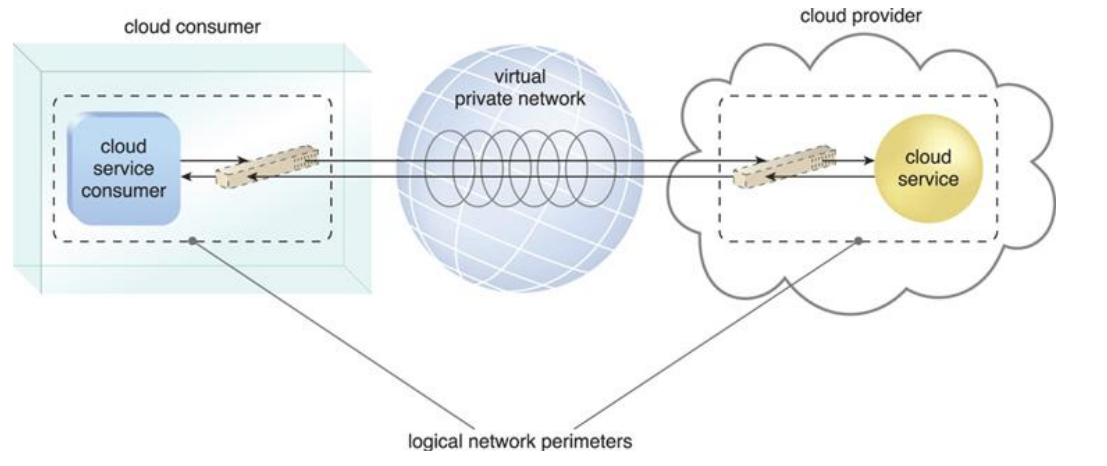
\includegraphics[width=8cm]{./Images/cap8/8.1.png}
\end{figure}

\subsubsection{\textbf{CASE STUDY: DTGOV}}
DTGOV, vista in precedenza, è un'azienda americana pubblica creata nel 1980 dal ministero della social security che permette di decentralizzare tutti i servizi informatici ad un'azienda indipendente ma a capitale pubblico. DTGOV virtualizza la sua infrastruttura di rete definendo un logical network perimeter che offre varie strutture:

\begin{figure}[htb!]
    \centering
    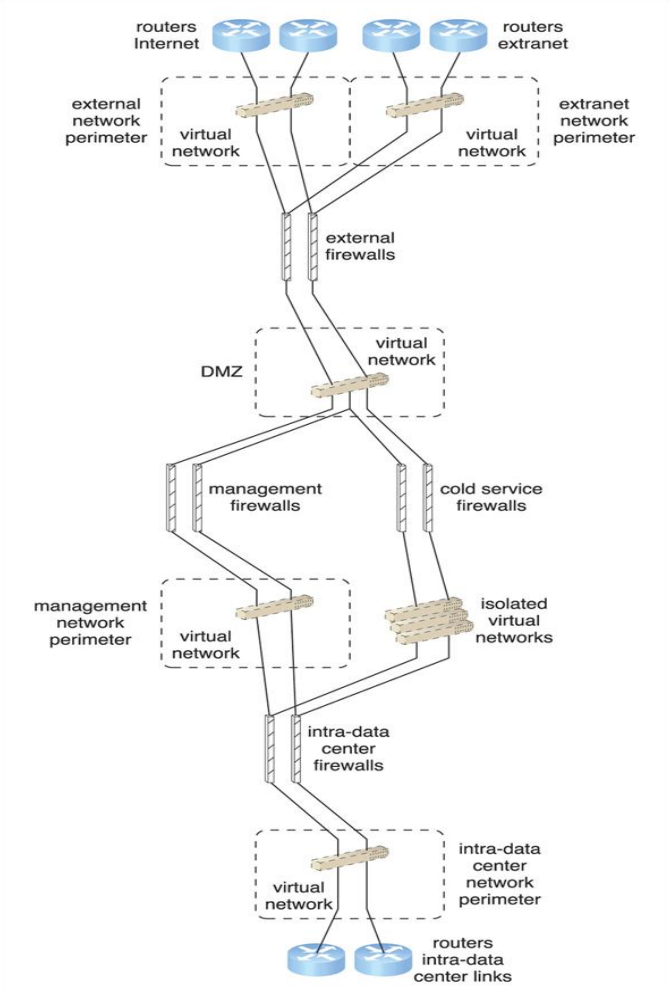
\includegraphics[width=8cm]{./Images/cap8/8.2.png}
\end{figure}

I router collegano il perimetro ad internet e extranet\footnote{\textit{Extranet} rappresenta una serie di intranet collegate per avere una rete aziendale distribuita ma privata.}. Un logical network perimeter è classificato come DMZ (\textit{demilitarized zone}): ci sono una serie di servizi necessariamente esposti all'esterno (come DNS o email) che si trovano in una parte attivamente protetta per separare i servizi esterni da quelli interni e capace di collegarsi con l'esterno.

Il traffico che passa nei firewall viene isolato entrando nella rete di management, che è la rete delle periferiche che si occupano di gestire il monitoraggio. Il traffico che va verso le risorse cloud passa attraverso la DMZ e nei firewall che isolano la parte dei servizi a cui il consumer può accedere. Per fare questo si passa dai router che forniscono i servizi di network perimeter attraverso i data center.

\vspace{5mm}

Questo tipo di architettura prevede risorse, management e DMZ. I firewall virtuali sono allocati per un singolo cloud consumer, in questo modo il consumer può regolare il suo traffico di rete virtuale in modo che sia isolato da tutti gli altri consumer.

\section{Virtual Server}
È una struttura di base che consiste nell'eseguire dei server virtuali che vengono forniti da server fisici. I server virtuali sono erogati come un bene di consumo, quindi possono essere acquistati e sono fondamentali per un ambiente cloud, perché le macchine virtuali sono rappresentate come file immagine, cioè un insieme di file che rappresentano la macchina virtuale in esecuzione, quindi risulta molto semplice crearne al voto o usarle durante l'esecuzione.

\subsubsection{\textbf{CASE STUDY: DTGOV}}
Le necessità computazionali vengono mappate su server virtuali. L'infrastruttura si basa su hypervisor che fungono da gestione e rendono il sistema leggero. Inoltre il sistema è coordinato da una Virtual Infrastructure Manager (VIM) che tramite gli hypervisor gestisce i vari server fisici. Questo approccio viene utilizzato in tutti i data center di DTGOV per assicurare l'uniformità.

\begin{figure}[htb!]
    \centering
    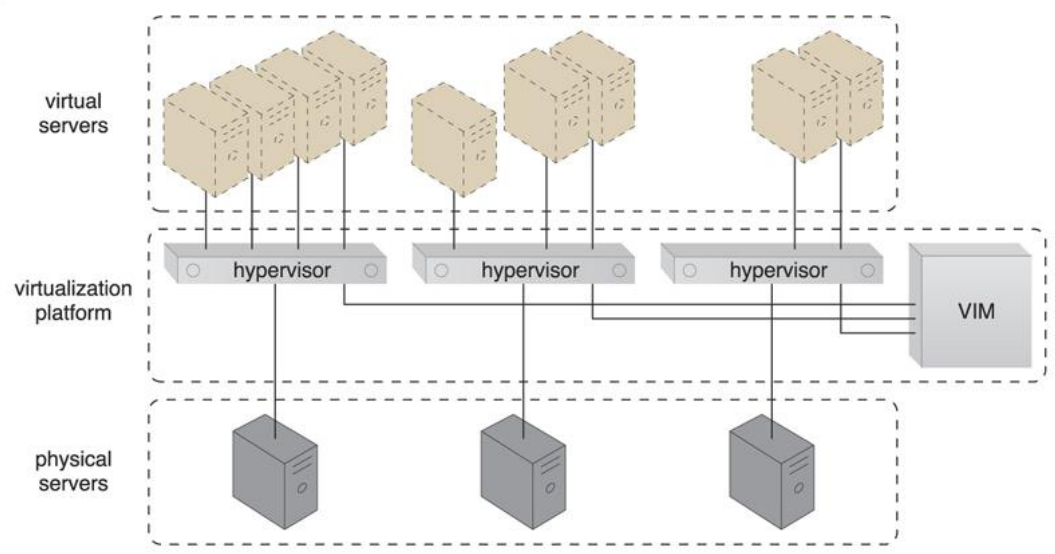
\includegraphics[width=9cm]{./Images/cap8/8.3.png}
\end{figure}

\section{Cloud Storage Device}
I device di storage vengono forniti esclusivamente via cloud ed esistono storage virtualizzati, allocati con un incremento fissato secondo un modello pay-per-use e vengono esposti attraverso i servizi. La situazione quindi è molto flessibile perché è possibile acquistare la taglia giusta di GB. I livelli di storage sono divisi in:
\begin{itemize}
    \item \textbf{File}: file e directory
    \item \textbf{Blocks}: il livello più basso fisicamente accessibile
    \item \textbf{Dataset}: organizzato in tabelle
    \item \textbf{Objects}: dati e metadati organizzati come risorse accessibili via web
\end{itemize}

\subsubsection{\textbf{CASE STUDY: DTGOV}}
Viene utilizzato un servizio che sfrutta metodi CRUD e la funzione di ricerca che usa una gerarchia di memorizzazione simile ad un filesystem, offrendo al contempo la creazione di cloud storage con un'interfaccia a blocchi. Il vantaggio di un'architettura object based è che lo storage sottostante ha capacità variabile a seconda della necessità degli oggetti da memorizzare. Inoltre è possibile creare device virtualizzati allocandoli a singoli consumer.

Ogni device ha un \textit{locial unit number} (LUN) che lo identifica e la creazione di un blocco viene fatta istanziando questa LUN sullo storage virtuale: questo serve alla VIM per assegnare una partizione al virtual server.

\begin{figure}[htb!]
    \centering
    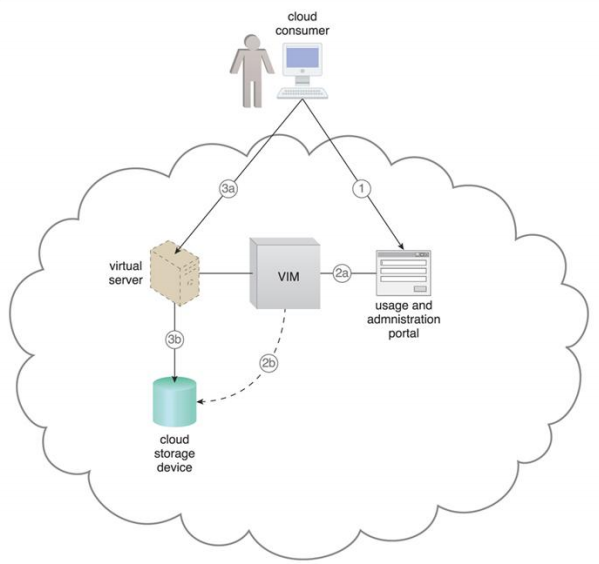
\includegraphics[width=8cm]{./Images/cap8/8.4.png}
\end{figure}

\section{Cloud Usage Monitor}
L'obiettivo è monitorare esattamente cosa sta usando il cloud. C'è una serie di monitor specifici per ogni servizio e queste statistiche vengono collezionate e mandate su un db per post processing o reporting. Ci sono tre implementazioni:
\begin{itemize}
    \item \textbf{MONITORING AGENT} - è un intermediario, cioè un programma guidato dagli eventi che risiede sul communication path per monitorare gli eventi e analizzare i dataflow. Il servizio viene fornito ma in maniera parallela la richiesta viene monitorata in un db di log.
    \item \textbf{REPORTING AGENT} - si trova più all'interno e si occupa di monitorare quello che avviene all'interno di un software, cioè c'è un'azione attiva da parte dell'agente che monitora il db. Viene usato per controllare le metriche basate su eventi osservabili come scaling verticale, inizializzazione o sospensione di un software.
    \item \textbf{POLLING AGENT} - fa in continuazione polling dei servizi per memorizzare i dati, monitora periodicamente lo stato delle risorse e verifica uptime e downtime. Utile per gestire le metriche stabilite dal SLA.
\end{itemize}

\subsubsection{\textbf{CASE STUDY: DTGOV}}
Servono misure accurate per evitare billing basato solo su server fisici a prescindere dall'utilizzo. Serve anche per stabilire il leasing dei server virtuali, legati ai vari livelli di performance, per macchine usate poco e macchine usate a pieno regime. Si implementa un resource agent che si occupa di monitorare tutti gli eventi generati dalla VIM per calcolare l'utilizzo delle macchine fisiche. Il periodo di misurazione inizia dalla creazione dei virtual server e si ferma alla loro terminazione.

\section{Resource Replication}
La replicazione delle risorse è uno degli strumenti più potenti per assicurare scaling e resilienza ai malfunzionamenti. Il meccanismo utilizzato è quello della virtualizzazione, con uno o più hypervisor che gestiscono diversi server e ognuno degli hypervisor può decidere di creare un certo numero di copie delle macchine che stanno sullo stesso device di storage fisico.

\subsubsection{\textbf{CASE STUDY: DTGOV}}
Due centri di calcolo sono collegati tra di loro attraverso un virtual private network (VPN). Il fatto che venga assicurata la replicazione delle risorse è importante perché in caso di malfunzionamenti la replica serve per poter effettuare la migrazione di uno dei server in un altro data center. La migrazione ovviamente è puramente virtuale.

\section{Ready-Made Environment}
È un meccanismo che fa parte del modello PaaS. pronto per essere utilizzato e può essere customizzato, in modo che il consumer possa utilizzare delle macchine pre-configurate. Tipicamente includono varie risorse come IDE, strumenti di gestione, ecc. Ci sono varie configurazioni a seconda delle esigenze, ad esempio una macchina che deve lavorare sul frontend avrà bisogno di infrastruttura di rete potente, mentre una macchina che lavora sul backend avrà bisogno di più risorse di calcolo. Queste istanze possono essere combinate per ottimizzare performance e costi.

\subsubsection{\textbf{CASE STUDY: ATN}}
Utilizza un ambiente PaaS, con applicazioni basate su Java per il catalogo dei magazzini che memorizza informazioni su switch e router. Questo tipo di software è usato da diverse factories ma non gestisce la parte delle transazioni. Fornisce delle istanze ready-made.

\vspace{5mm}

Una volta affrontati tutti i meccanismi, possiamo mapparli con le caratteristiche del cloud definite dal NIST:

\begin{table}[htb!]
\centering
\begin{tabular}{|c|c|} 
\hline
\begin{tabular}[c]{@{}c@{}}\\Logical Network Perimeter\\\end{tabular} & \begin{tabular}[c]{@{}c@{}}Ubiquitous Access, Multitenancy/Resource \\Pooling\end{tabular}                        \\ 
\hline
\begin{tabular}[c]{@{}c@{}}\\Virtual Server\\\end{tabular}            & On-demand Usage                                                                                                   \\ 
\hline
\begin{tabular}[c]{@{}c@{}}\\Cloud Storage Device\\\end{tabular}      & Elasticity                                                                                                        \\ 
\hline
\begin{tabular}[c]{@{}c@{}}\\Cloud Usage Monitor\\\end{tabular}       & Elasticity, Measured Usage                                                                                        \\ 
\hline
\begin{tabular}[c]{@{}c@{}}\\Resource Replication\\\end{tabular}      & \begin{tabular}[c]{@{}c@{}}On-demand Usage, Multitenancy/Resource Pooling, \\Elasticity, Resiliency\end{tabular}  \\ 
\hline
\begin{tabular}[c]{@{}c@{}}\\Ready-Made Environment\\\end{tabular}    & On-demand Usage                                                                                                   \\
\hline
\end{tabular}
\end{table}

\section{Learning Check}
\begin{enumerate}
    \item Descrivi l'obiettivo del meccanismo del Logical Network Perimeter e come esso definisce un limite logico.
    \item Elenca le componenti usate comunemente per costruire un Logical Network Perimeter.
    \item Descrivi il meccanismo del virtual server e spiega la differenza tra un server virtuale e un server fisico e come è configurato l'ambiente di virtualizzazione.
    \item Descrivi l'obiettivo del meccanismo del Cloud Storage Device.
    \item Elenca le componenti che possono essere usate per esporre o garantire l'accesso ai dispositivi di cloud storage.
    \item Descrivi l'obiettivo del meccanismo del Cloud Usage Monitor ed elenca i meccanismi che sono considerate variazioni specializzate.
    \item Elenca e spiega le tre implementazioni iutilizzate per i Cloud Usage Monitor.
    \item Descrivi il meccanismo del Resource Replication e come si relaziona con il meccanismo dell'hypervisor.
    \item Descrivi il meccanismo del Ready-Made Environment e spiega le risorse IT che fornisce, le sue relazioni con il modello di delivery PaaS e come può esistere su un server fisico o virtuale.
\end{enumerate}
